يقدم هذا القسم مجمل ما تم مراجعته بهدف تصميم وتنفيذ خوارزمية البحث والمنصّة الفعالة.

\subsection{التصنيف والتصميم}

إنّ الأنظمة متعدّدة الروبوتات تلاقي اهتماماً كبيراً في المراجع ولاسيّما في الآونة الأخيرة؛ نظراً إلى أنّ مجالات التّطبيق والمهام الّتي تواجهها تزداد تعقيداً. لقد تمّ اقتراح تصنيف جديد في عام 2004 اعتماداً على ثلاث نقاط أساسيّة: (1) عقلانيّة التّصميم، (2) الوظائف التّقنيّة الاساسيّة (لكّل من العتاد الصّلب والبرمجيّات)، (3) المهمّات الّتي يجب أن تقوم الرّوبوتات بتنفيذها. حيث تمّ التّصنيف على عدّة مستويات ضمن فئتين أساسيّين: الأبعاد التنسيقيّة، وأبعاد النّظام كما هو موضّح في الجدول \ref{06:table:1} \cite{b4}. 

\begin{table}[]
	\begin{tabular}{|l|l|}
		\hline
		الأبعاد التّنسيقيّة Coordination Dimensions & أبعاد النّظام System Dimensions       \\ \hline
		التّعاون   Cooperative                      & الاتّصال   Communication              \\ \hline
		المعرفة Knowledge                           & تكوين   الفريق team Composition       \\ \hline
		التّنسيق   Coordination                     & هيكليّة   النّظام System Architecture \\ \hline
		التّنظيم Organization                       & حجم الفريق Team Size                  \\ \hline
	\end{tabular}
\caption{الأبعاد التنسيقية وأبعاد النظام}
\label{06:table:1}
\end{table}

وفي العام التّالي طرحت الورقة البحثيّة \cite{b5} تبين أنّ أي فعل يقوم به أي روبوت يَأخذ بالحسبان الأفعال الّتي تقوم بها بقيّة الرّوبوتات، وهكذا ينتج مجموعة من الرّوبوتات الّتي تعمل باتّساق لتحقيق أفضل أداء ممكن. وقد أظهرت هذه الآليّة من التّنسيق أداء عالٍ؛ حيث تمكّنت الروبوتات من اكتشاف بيئتها في وقت أقل مقارنةً مع المنهجيّات الأخرى الّتي لا تعتمد على التنسيق بين الرّوبوتات بشكل صريح. وبالرّغم من النّتائج الجيّدة الّذي حقّقها النّهج المتّبع في البحث \cite{b5}، إلّا أنّ هناك بعض النقاط الّتي تحتاج إلى تطوير، حيث يجب مناقشة الحالات الّتي يتمّ فيها تعطّل أحد الرّوبوتات أو حدوث تغيّر ما في البيئة المحيطة بها.

ومن ناحية أخرى، نالت أعداد الرّوبوتات الّتي تشكّل السّرب اهتماماً كبيراً في مجال البحث العلميّ. على الرّغم من أنّ سلوك كلّ روبوت على حدا يُعدّ سلوكاً بسيطاً، إلاّ أنّه عندما تعمل هذه الرّوبوتات معاً يصبح سلوكها أكثر تعقيداً. أشار \cite{b6} إلى أنّ فهم الرّوبوتات بشكل فرديّ هو أمرٌ سهل، أمّا بالنّسبة لتوقّع سلوكها معاً فهو أمرٌ صعب المنال. لقد تمّ عرض النّهج المعتمد من قبل \cite{b6} من خلال التّحليل العميق لخوارزميّة السّرب المُتّبعة والنّموذج الاحتمالي المُرتبط بها؛ حيث تمّ فحص خوارزميّة التّحكم باستخدام فضاء الحالة المُطوّرة من قبل \cite{b7} على مجموعة من الرّوبوتات الباحثة عن طعام.


 لقد قام \cite{b6} باستخدام خوارزميّة ألفا في شبكة الاتّصال اعتماداً على المنطق الزّمني $ (Temporal logic) $، حيث تمّ التّركيز على حالة الرّوبوتات بدلاً من الموقع وتفاصيل حركة كلّ روبوت. ولكنّ وبالرّغم من النّتائج المُرضية وصل اليها البحث، إلا أنه لم يتمكّن من إجراء عملية التّحليل سوى على عدد قليل من الرّوبوتات بسبب مشكلة انفجار الحالة $ (state explosion) $ التي ظهرت أثناء عمليّة فحص النّموذج الرّياضي. 
 
 \subsection{تخطيط المسار}
 
 تُعدّ مشكلة تخطيط المسار متعدد الروبوتات مشكلة معقدة حسابياّ لأنّ صعوبة الحساب تنمو مع عدد الروبوتات. إنّ وجود قيود وعوائق في المسار يولّد مشكلة كبيرة، ومن هنا بدأت عمليّة البحث عن خوارزميّات لحلّ هذه المشكلة. أحد الخوارزميّات المُتّبعة لحلّ مشكلة المسار المقيّد هي الـ \textenglish{Visibility Graph (VG)}. تبدأ هذه الطريقة بتشكيل الرّسم البياني عن طريق رسم العقد (Nodes) والحواف (Edges) باستخدام تقنيّة التّصوير بالأشعّة، ومن ثمّ تحديد البيان الموجّه. يتمّ بعد ذلك إيجاد المسار الأقصر باستخدام خوارزميّات إيجاد الطريق الأقصر في البيان. نذكر هنا أن المسار النّاتج عادةً قريب جدّاً من العوائق.
 
 وكان البحث \cite{b8} قد قدّم عام 1985 طريقة فريدة لتفادي العوائق اعتماداً على تقنيّة الـ $ (Potential Field) $، حيثُ تمّ التّحكم بالروبوتات على عدّة مستويات وبالزّمن الحقيقي. وتتميّز هذه الطريقة بإمكانيّة توسيع الحلّ ليشمل البيئات ذات العوائق المُتحرّكة باستخدام حقل كموني متغيّر مع الزّمن.  وفي عام 2006 قدّم العمل \cite{b9} طريقة حقل كموني لتخطيط مسار الروبوت بالاعتماد على ناتج جمع تابعين هما: تابع $ (repulsive) $ الذي يتجنب المسارات القريبة من العوائق، وتابع $  (Attractive) $ قيمته تتعلق بالمسافة عن الهدف.
 
 إنّ طريقة الـ $ potential field $ هي طريقة مباشرة لحساب الحقل المتجهات $ (vector field) $ اعتماداً على موقع الهدف والعوائق، ولكنها تتطلّب روبوتات مُتحكّم بها بشكل كامل (قادرة على التّحرك بأي اتّجاه بشكل آني). على خلاف الحقل الكموني، طرق تخطيط المسار المعتمدة على الدّوال التّدفقيّة $ Stream function $ لا تتطلب التّحكم ذلك، كما أنّها تضمن تحوّل جميع نقاط التّوازن إلى نقاط سرجيّة، مما يعني ضمان وصول الروبوت إلى هدفه. لقد أظهرت عمليّة تخطيط المسار المُعتمدة على الدّوال التّدفقيّة المطروحة في \cite{b10} فعاليّة وسرعة عاليّة في التّكيف مع التّغيرات في الشّروط. على عكس طرق تخطيط المسار الأخرى، الطّرق الّتي تعتمد على الدّوال تتميز بمظهرها الحدسيّ بالنّسبة لمراقب الخارجي. إنّ وجود أكثر من حاجز لا يضمن دائماً الحصول على نتائج صحيحة، لكن هذا المثال يوضّح أن السلوك لا يزال مقبولاً كما هو موضح في الشكل \ref{06:fig:1}.
 \begin{figure}[h]
 	\centering
 	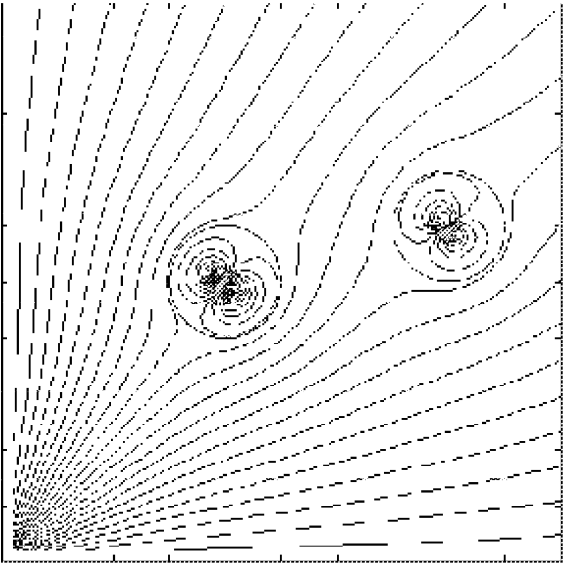
\includegraphics[width=0.5\linewidth]{figs/06/fig1}
 	\caption{مثال على الدوال التدفقية}
 	\label{06:fig:1}
 \end{figure}


في عام 2015 تمّ طرح سلالات فورونوي \textenglish{VORONOI STRAINS} كخوارزميّة جديدة لتخطيط المسار والّتي حقّقت فائدة مهمّة على صعيد البيئات المعقّدة \cite{b9}. لقد حقّقت هذه الخوارزميّة نتائج مثيرة للاهتمام في مساحات عمل فيها عدد كبير من العوائق، فقد أظهرت حلولاً أفضل بكثير من خوارزميّة PSO البسيطة والمُطوّرة من أجل نفس عدد التّكرارات. إضافة إلى ذلك، أثبتت أنّها أكثر صلادة وأقل اعتماديّة على الحالة الابتدائيّة (العشوائية). كما تتميّز هذه الخوارزميّة باحتماليّة أكبر لتجنّب النّقاط الصّغرى المحليّة، ولكن قد أثبتت التّجارب أن عمليّة االأمثلة هذه غير مُجدية مالم تكن البيئة معقّدة بشكل كافِ.

أثناء تخطيط الحركة يمكننا تصنيف العمل إلى صنفين أساسيّن؛ فإمّا أن يتمّ تخطيط المسار بشكل كامل قبل البدء بالحركة (offline)، أو أن تتمّ عمليّة التّخطيط بشكل تدريجي أثناء الحركة (online).

 
  في \cite{b11} ، تم التّركيز على تخطيط المسار بشكل كامل قبل بدء الحركة، بالإضافة إلى وجود حواجز ثابتة، وهي إحدى الأمور الّتي أعطت هذا البحث محدوديّته. تتميّز طريقة تخطيط المسار المُقترحة في \cite{b11} بأنّها تمكّننا من الحصول على مسار ثلاثي الأبعاد مثالي يمكن الروبوتات من التحليق على ارتفاعات منخفضة في بيئة ذات تضاريس مُعقّدة.
  
  وفي عام 2020 طُرحت الورقة البحثيّة \cite{b12} بهدف توجيه روبوتات طائرة في مجال جوّي مفتوح وتضاريس غير معلومة لتتفوق بذلك على البحث \cite{b11} وذلك عبر حلّ معادلة الاستمراريّة للموائع. لقد حقّقت هذه الدّراسة وقتاً أقلّ من أربع طُرق أخرى $( A*, Dijkstra, DP, PE) $.
  
  إضافة إلى الخوارزميات التقليدية، العديد من الدراسات أظهرت نتائج خوارزميات التعلم الآلي لحل هذه النوع من المشكلات. في \cite{c1} تم استخدام الشبكات العصبونية الالتفافية لتحسين حلول الخوارزميات التقليدية كما نجد في \cite{c2} أنه تم استخدام خوازرمية تعلم Q-learning معتمدة على الخوارزمية المحسنة \textenglish{improved particle swarm optimization}. تهدف الخوارزميات المستخدمة الى تقليل طول المسار وزمن الوصول وزوايا دوران الروبوتات لتقليل استهلاك الطاقة. تمت المقارنة بين اربع خوارزميات وايجاد النتائج باختلاف عدد الروبوتات في السرب هي CQL و PSO وIPSO-DV  و QIPSO-DV وأظهرت النتائج تفوق QIPSO-DV على باقي الخوارزميات كما يمكن ملاحظة تراجع أداء هذه الخوارزمية مع زيادة عدد الروبوتات ولاسيما من حيث زمن التنفيذ وعدد التكرارات اللازمة للوصول الى الحل الأمثل (إن وجد) .
  في \cite{c3} تم اقتراح تقسيم الخريطة الكلية الى خرائط بيان جزئية sub-graphs مع قيود على الدخول والخروج من كل خريطة وذلك لضمان إيجاد المسار. بعد التجريب، تم التوصل الى حل فعال وسريع نسبيا لكنه لا يضمن ايجاد مسار أمثل وبحاجة إلى عمليات معالجة لاحقة لتقليل المسافات الضائعة.  
  
   يعد موضوع انشاء طريق باستخدام الحل الرقمي للمعادلات التفاضلية الجزئية موضوع حديث عالمياً ويحتاج الكثير من العمل، قدمت واحدة من الأبحاث القائمة على موضوع استغلال جريان السوائل في توليد المسار عام 2017، حيث تهدف \cite{b13} الى انشاء المسار الأفضل لحركة سفينة باستخدام طريقة $ lattice Boltzmann $ الرقمية. البحث لم يناقش آلية انشاء طريق من نقطة إلى اخرى في فضاء العمل، بل ناقش عبور منطقة تحتوي عوائق بشكل عام. إضافة لذلك، فإن الحل الرقمي باستخدام $ lattice Boltzmann $ لم ينتج حقول متجهات سرعة تحمل نفس السلوك الفيزيائي للسوائل، يمكن التحقق من ذلك بالنظر في سلوك الحقل عند الحواجز في الشكل \ref{06:fig:2}.
   
         
   \begin{figure}[htbp]
   	\centering
   	\includesvg[width=0.85\linewidth]{figs/06/fig06_2}
   	\caption{التدفق المولد باستخدام الخوارزمية $ lattice Boltzman $. يمكن ملاحظة السلوك غير الفيزيائي للسائل بالنظر الى تداخل السائل مع الجدران.}
   	\label{06:fig:2}
   \end{figure}
   
   
      
      وكان قد طُرح في عام 2009 نظام  قوي وسريع لتخطيط المسار للملاحة الآليّة \cite{b14}، والفكرة الأساسيّة الّتي اعتمد عليها هذا البحث هي انشاء المسار عبر نشر موجتين متتاليتين، كما في الشكل \ref{06:fig:3}. تبدأ بموجة أولى تكون ذات سرعة قليلة نسبيّاً تُمكّن الرّوبوت من نقل طوبولوجيا الخريطة إلى الحاسوب، بينما تنتقل الموجة الثّانية ذات السّرعة العالية في الخريطة وذلك من أجل تكوين مسار من نقاط جهات الانتشار ذات التّقعّر الأعلى. وفي النّهاية يمكن التّحكم في المسارات المثلى المخطّطة اعتماداً على معامل واحد: المسار الأقصر، الأكثر أماناً، أو الهجين.
       \begin{figure}[h]
      	\centering
      	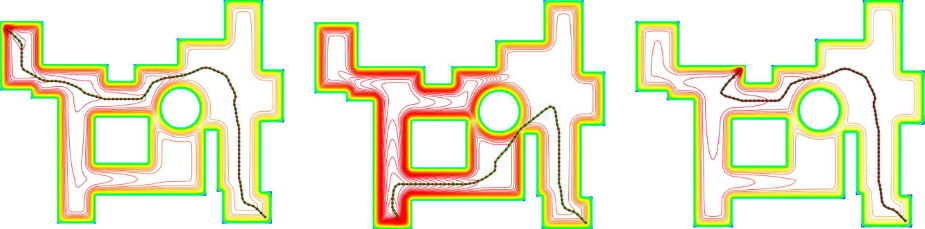
\includegraphics[width=0.9\linewidth]{figs/06/fig06_3}
      	\caption{الأمواج المتقدمة والمتأخرة في العمل\cite{b14}}
      	\label{06:fig:3}
      \end{figure}
      
      
      \subsection{الاتصال}
      
      كما أشرنا سابقاً، فإنّ فكرة الاسراب مأخوذة من الأسراب البيولوجيّة، حيث أن أساس التّحكم في سلوك هذه الأسراب هو تبادل المعلومات. يتمكّن الأفراد في الاسراب البيولوجيّة من تبادل المعلومات بشكل مباشر عن طريق المجسّات، الحركة، أو الصّوت. استوحى \cite{b15} تصنيف أسراب الرّوبوتات من الاسراب البيولوجيّة، حيث تمّ التّصنيف إلى مجموعتين أساسيّتين:
            
      \begin{itemize}
      	\item \textbf{أولاً: التّفاعل عن طريق التّحسس:} هو الطّريقة الأبسط للتّواصل بين الرّوبوتات. تتطلّب من الرّوبوت التّمييز بين الأقران والبيئة المحيطة به. يطلق على هذا النّوع من الاتّصال بالصّريح. 
      	\item \textbf{ثانياً: التّفاعل عن طريق البيئة:} حيث تستخدم الرّوبوتات البيئة كوسيلة للتّواصل فيما بينها. يسمّى هذا النّوع بالتّواصل الضّمني. أسراب النّمل مثال شهير على الاتّصال الضّمني؛ حيث يتواصل أفراد السّرب عن طريق إفراز وتتبع مادّة الفيرومون \cite{b15}.
      \end{itemize}
      
      هناك العديد من طرق الاتّصال المستخدمة في أسراب الروبوتات، ومن التّقنيات المستخدمة للاتصال بين الرّوبوتات في السّرب الواحد (الأشعة تحت الحمراء، البلوتوث، الـWi-Fi، ZigBee، ...). تعد عمليّة اختيار التّقنيّة المناسبة مهمّة جدّاً لأنها مؤثر مباشر على أداء السرب، لذلك تتمّ بناءً على عدّة معايير (البيئة الّتي تعمل بها الرّوبوتات، مدى الاّتصال، معدّل نقل البيانات، ...) وقد قام العمل \cite{b16} بمقارنة أداء هذه الطّرق.
      
وعندما نتوجّه نحو الاتّصال اللاسلكي فإنّ شرائح الـ ESP8266 توفر ما يجعلها الخيار الأمثل، فهي منخفضة التّكلفة مقارنة بأدائها، وتدعم بروتوكولات TCP/IP بشكل كامل.  تتكون من SoC يحوي معالج Xtensa Tensilica [32bit]  وشريحة Wi-Fi تدعم بروتوكول  الاتّصال اللاسلكي IEEE 802.11b/g/n،  اضافة إلى العديد من الميّزات كما ورد في مقدّمة \cite{b17}.

مجتمع الـ Opensource الخاص بشريحة الـ ESP وفّر مكتبة PainlessMesh المبنية خصّيصاً لتشكيل شبكات تعتمد على أجهزةESP8266؛ حيث أنّها تبني شبكة خالية من الحلقات وتقوم بالتّحديث كلّ 3 ثواني. إلّا أنّه ومع الأسف كان هنالك انخفاض ملحوظ في أداء الشّبكة مع ازدياد العقد المُتّصلة بها كما كان واضحاً في نتائج التّجارب الّتي قام بها \cite{b17}.


بصورة عامة، تكمن الغاية الأساسية من تصنيع وتركيب الروبوتات بشكل عامة في الوظيفة التي ستقوم بها على أرض الواقع، ومن هنا يصبح للتنفيذ الفعلي أهمية كبيرة حيث أن محاكاة أداء الروبوتات ومهما كان دقيقا، فإنه يستخدم فقط لتقييم التصميم قبل التنفيذ الفعلي.
عالمياً، نجد تنوع كبير في منصات أسراب الروبوت وفق الغاية منها، بعضها تكون لأهداف تعليمية والبعض الآخر لأهداف بحثية لختبار صحة الخوارزميات كما في بحثنا هذا. تقدم \cite{c4} مراجعة عامة لأهم وأشهر منصات أسراب الروبوت ومقارنة من حيث الخصائص العامة والحجم والسعر والحساسات المستخدمة. تم التوصل إلى أن معظم هذه المنصات مناسبة جدا للأغراض البحثية، كما أن بعض المنصات مثل MarXbot وsbot وPheeno مناسبة للاستخدام على أرض الواقع وذلك لمرونة التصميم وإمكانية عبورها ضمن البيئات الصعبة. نجد في الجدول ملخصاّ عن المقارنة بين المنصات.

\begin{table}[]
	\begin{tabular}{@{}lp{10pt}p{10pt}p{10pt}r@{}}
		\toprule
		& التكلفة (دولار)          & الحجم (سم)               & عمر البطارية (ساعة)   & \multicolumn{1}{c}{الخصائص المميزة}                                                     \\ \midrule
		Colias \cite{c5}   & 25                      & 4                        & 4                     & وحدة استشعار بالأشعة تحت الحمراء ذات مدى   طويل                                         \\
		AmiR \cite{c5}    & 65                      & 6.5                      & 2                     & حساسات ذات درجة حساسية عالية                                                            \\
		Kilobot \cite{c6}  & 14                      & 3.3                      & 3                  & دواليب ذات حركة بنمط Omni                                                               \\
		R-one \cite{c7}     & 220                     & 10                       & 6                     & قابلة للتغير بشكل ذاتي، آلية اقتران                                                     \\
		s-bot \cite{c8}    & -                       & 15                       & 1                     & آلية اقتران، قابلية تجمع بشكل ذاتي،   كاميرا متحركة بكل الاتجاهات                       \\
		e-puck \cite{c9}    & 1200                    & 75                       & 2                     & يمكن محاكاتها باستخدام محاكي WEMBOTS و ENKI                                             \\
		MarxBot \cite{c10}  & -                       & 17                       & 8                     & قابلة للتغير بشكل ذاتي، آلية اقتران،   كاميرا متحركة بكل الاتجاهات، تصميم ببنية معيارية \\
		Pheeno \cite{c11}   & \multicolumn{1}{l}{270} & \multicolumn{1}{l}{12.7} & \multicolumn{1}{l}{-} & آلية قبض، كاميرا                                                                        \\ \bottomrule
	\end{tabular}
\end{table}